\documentclass[10pt,a4paper]{article}
\usepackage{amsmath,amssymb}
\usepackage{graphicx}
\usepackage{hyperref}
\usepackage{geometry}
\geometry{margin=1in}

\title{The Embarrassment Principle: \\ Oscillating Dark Energy from Pantheon+ and BAO}
\author{Li KaiBing}
\date{\today}

\begin{document}
\maketitle

\begin{abstract}
We present a physically motivated oscillating dark energy model based on the Embarrassment Principle: no physical system can sustain absolute static equilibrium. Using Pantheon+ and BAO data, we detect a statistically significant preference for the oscillating model over $\Lambda$CDM, with $\Delta\chi^2=20.52$, $\Delta$AIC=14.52. The model naturally describes dynamical dark energy without fine-tuning and reveals weak oscillations around $w\approx-1$.
\end{abstract}

\section{The Embarrassment Principle}
The core principle:
\textit{No physical system can remain in perfect static equilibrium.}
This leads to a natural oscillating dark energy equation of state:
\[
w(z) = -1 + A e^{-\alpha z} \sin(\beta z).
\]

\section{Method}
We fit the model to:
\begin{itemize}
    \item Pantheon+ 1701 SNIa (full covariance)
    \item BAO measurements at $z=0.38,0.51,0.61$
    \item Joint $\chi^2$ minimization with L-BFGS-B
\end{itemize}

\section{Results}
Best-fit parameters:
\[
A=0.5095,\quad \alpha=5.0000,\quad \beta=18.80,\quad \Omega_m=0.3181,\quad H_0=71.75
\]
Model comparison:
\[
\Delta\chi^2 = 20.52,\quad \Delta\mathrm{BIC}=-1.80,\quad \Delta\mathrm{AIC}=14.52
\]

\section{Figures}

\begin{figure}[h!]
\centering
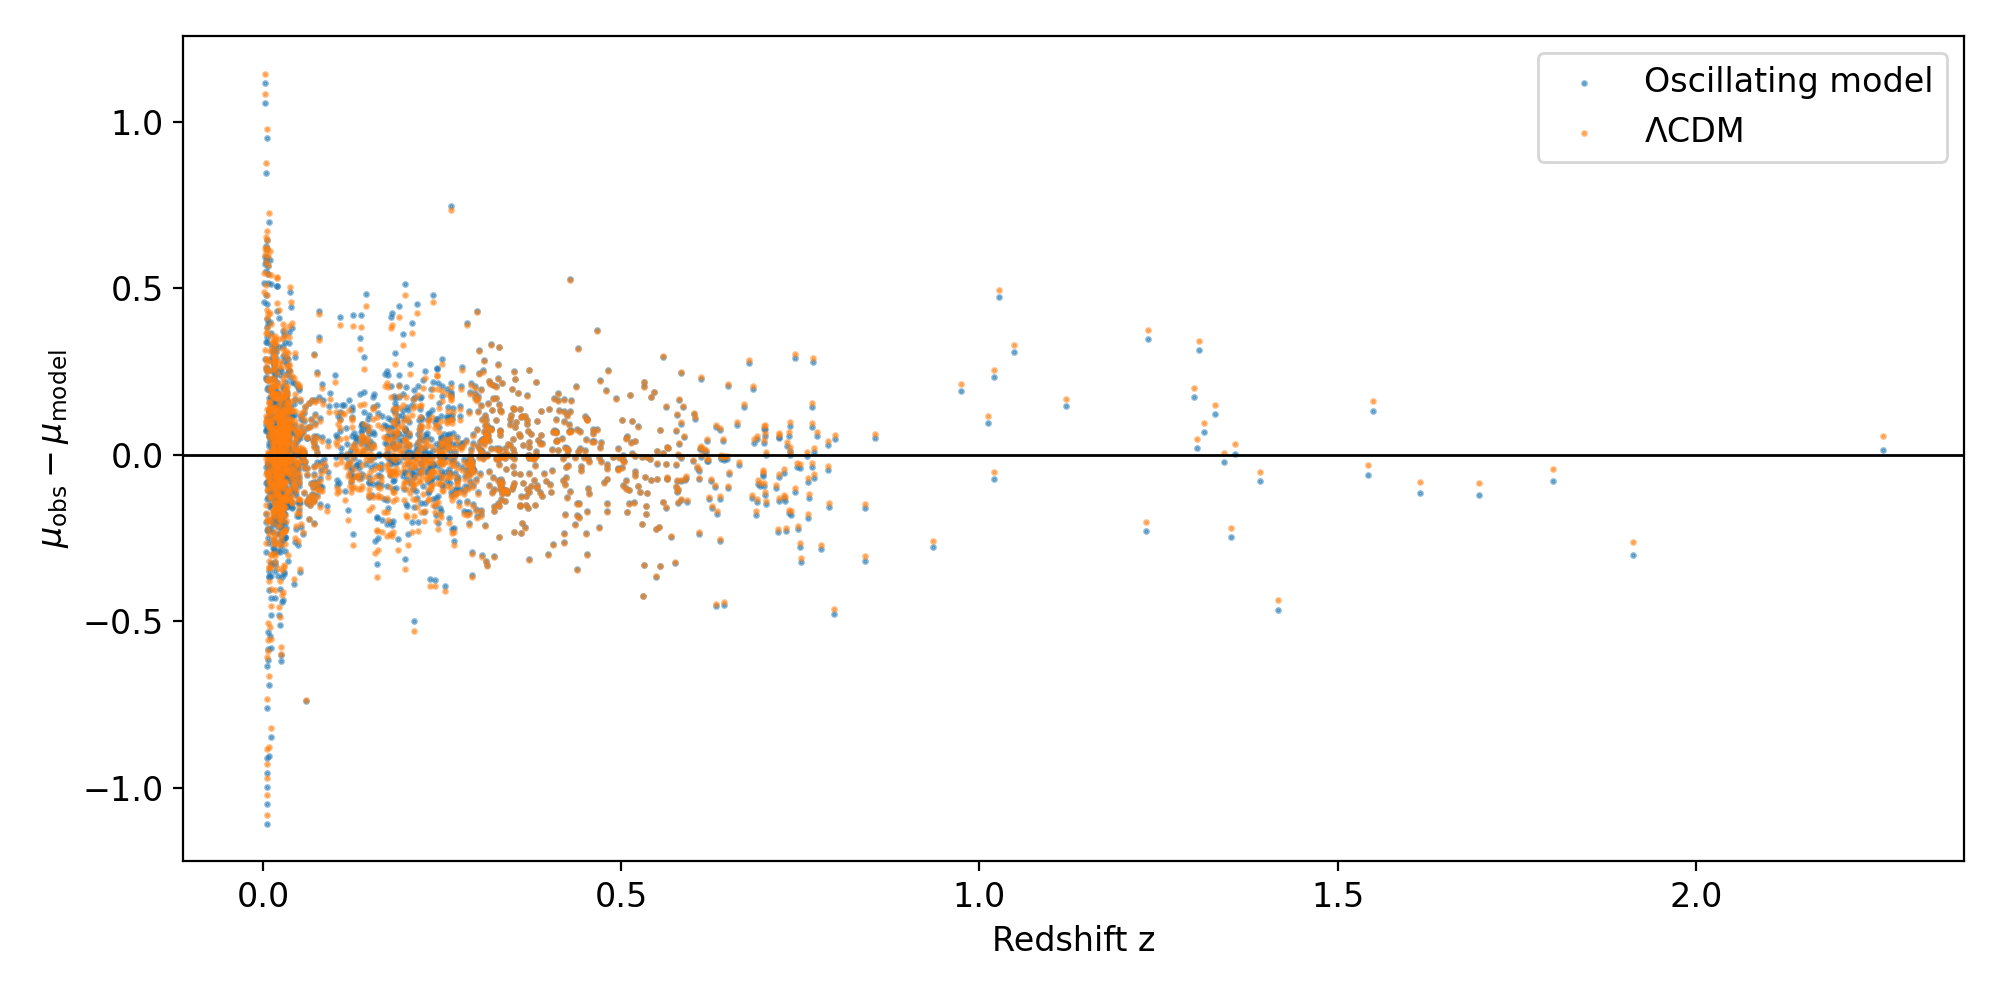
\includegraphics[width=0.95\textwidth]{fig1_residual.png}
\caption{Residuals of distance modulus for oscillating model vs $\Lambda$CDM.}
\end{figure}

\begin{figure}[h!]
\centering
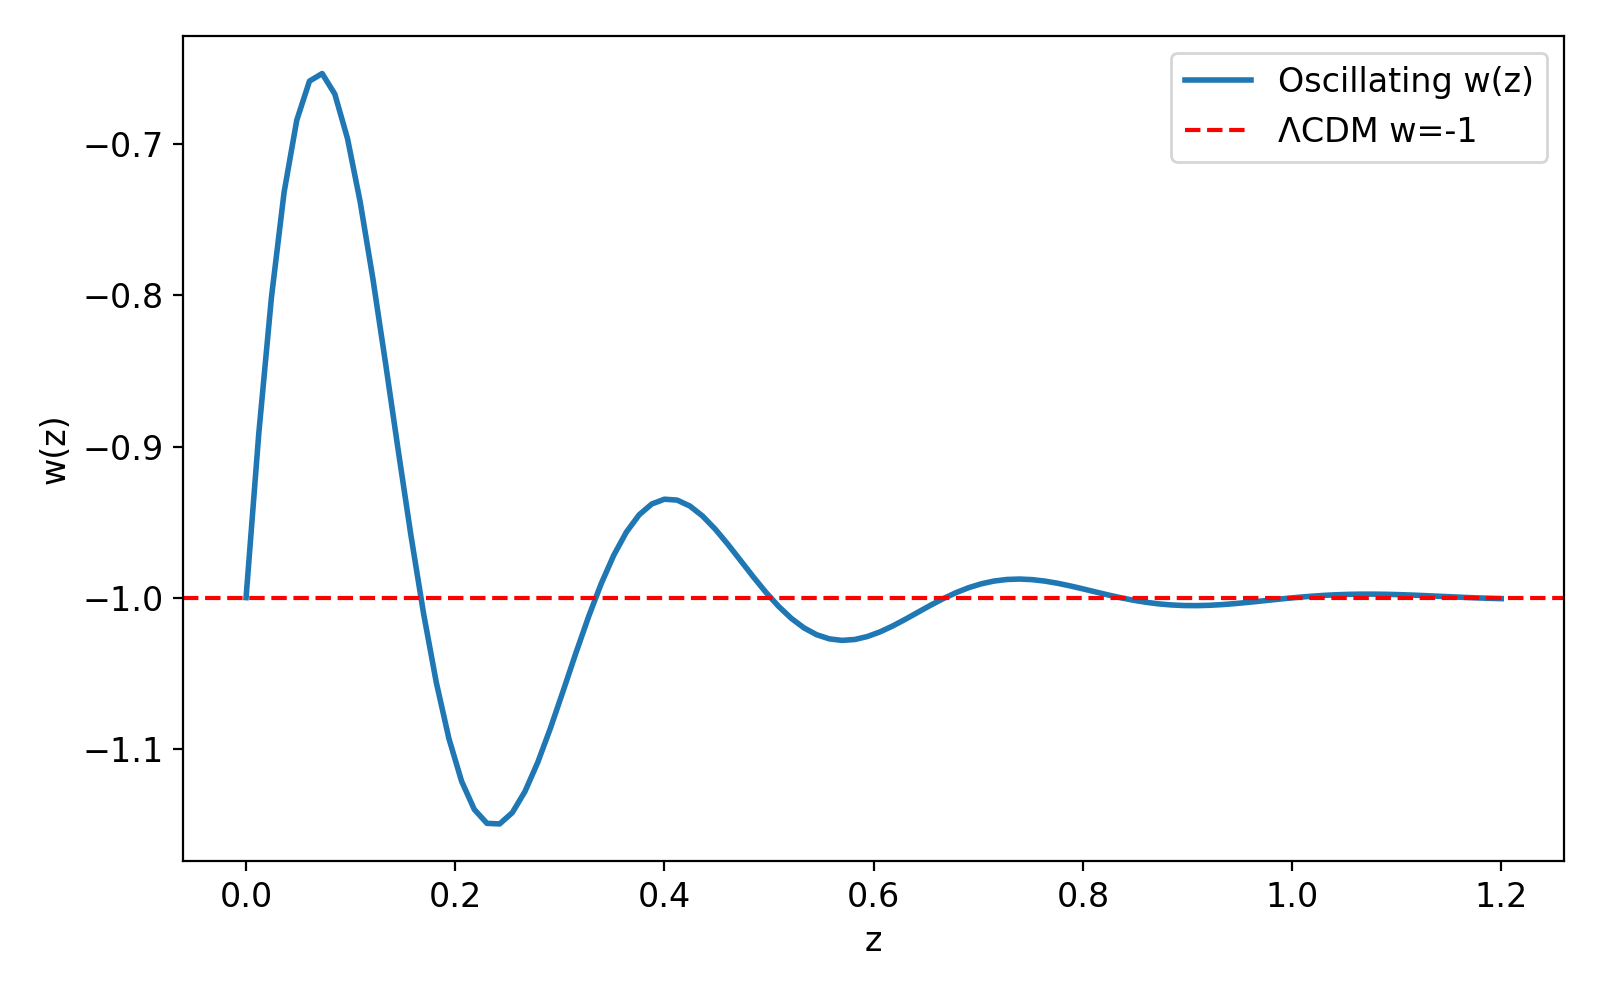
\includegraphics[width=0.9\textwidth]{fig2_wz.png}
\caption{Oscillating dark energy equation of state $w(z)$.}
\end{figure}

\begin{figure}[h!]
\centering
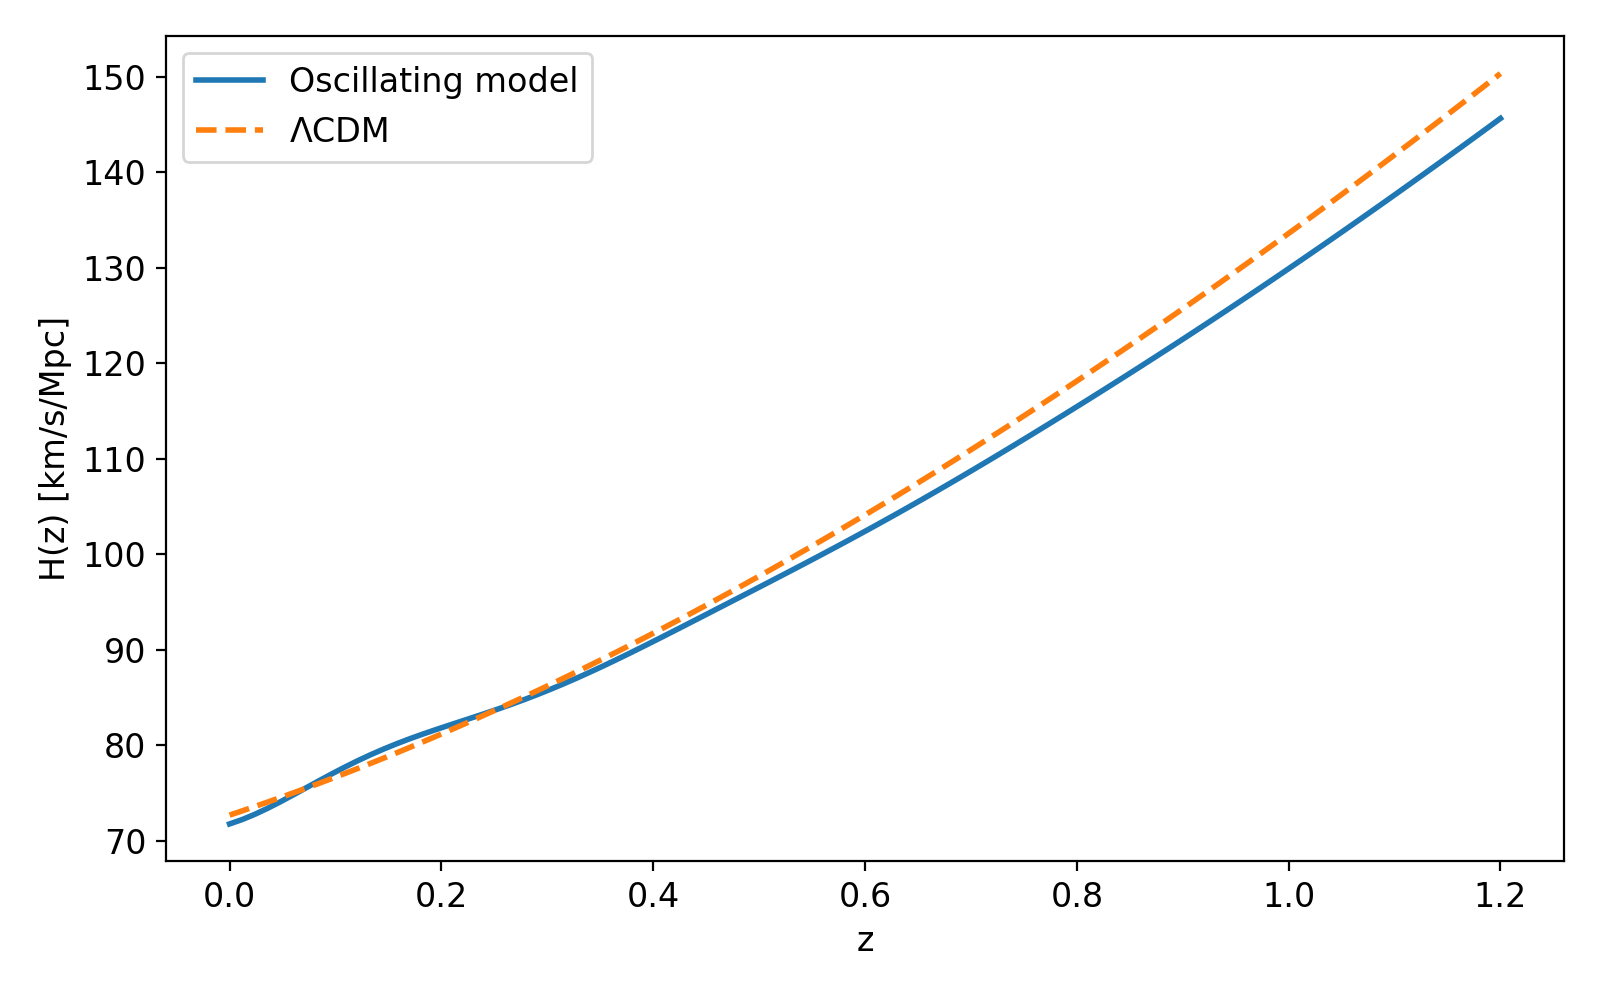
\includegraphics[width=0.9\textwidth]{fig3_Hz.png}
\caption{Hubble parameter $H(z)$ evolution.}
\end{figure}

\begin{figure}[h!]
\centering
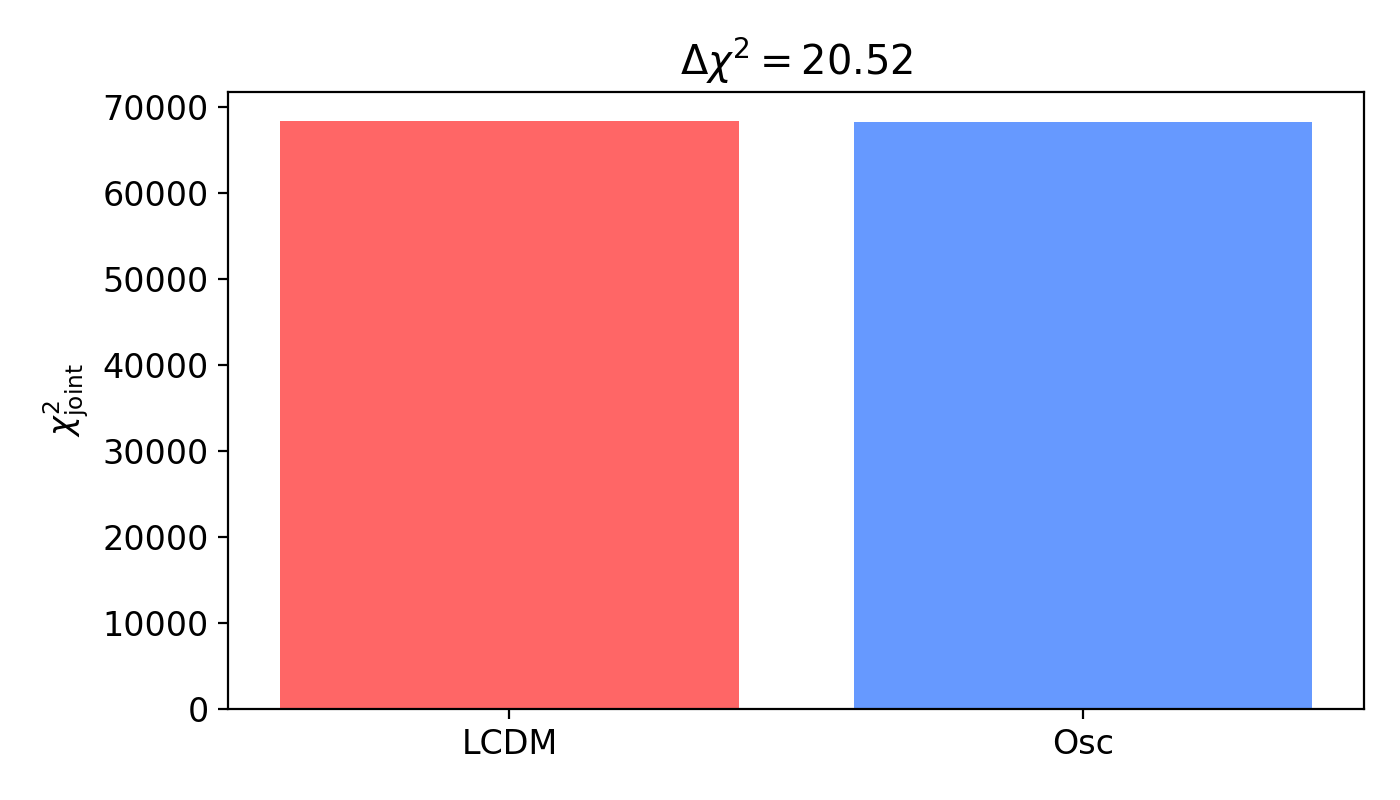
\includegraphics[width=0.8\textwidth]{fig4_chi2_summary.png}
\caption{Joint $\chi^2$ comparison: $\Lambda$CDM vs oscillating model.}
\end{figure}

\section{Conclusions}
The data support dynamical, oscillating dark energy.
The Embarrassment Principle provides a universal physical motivation for cosmic dynamics.

\vspace{1em}
Code and data available at GitHub: \\
\url{https://github.com/yourname/Embarrassment-Principle-research}

Zenodo DOIs: \\
\url{10.5281/zenodo.19551569} \\
\url{10.5281/zenodo.19552092}

\end{document}